\documentclass[aspectratio=169]{beamer}



% OPCIONES DE BEAMER

\definecolor{Maroon}{cmyk}{0, 0.87, 0.88, 0.1}
\definecolor{teal}{rgb}{0.0, 0.45, 0.45}

\usetheme[block=fill,numbering=fraction,, subsectionpage=progressbar, titleformat section=smallcaps]{metropolis}
\setbeamertemplate{blocks}[rounded][shadow=false]
\setbeamertemplate{frametitle continuation}[roman]
\setbeamertemplate{section in toc}[balls numbered]
\setbeamertemplate{subsection in toc}[subsections unnumbered]
%\setsansfont[BviejoFont={Fira Sans SemiBold}]{Fira Sans Book}  % Increase font weigth
\widowpenalties 1 10000
\raggedbottom

% COLORES
\setbeamercolor{palette primary}{bg=teal}
\setbeamercolor{progress bar}{use=Maroon, fg=Maroon}

% PAQUETES
\usepackage{bm}
\usepackage{xcolor}
\colorlet{shadecolor}{blue!15}
\usepackage{framed}
\usepackage{amsthm}
\usepackage[utf8]{inputenc}
\usepackage[english]{babel}
\usepackage{subfig}
\usepackage{graphicx}
\usepackage{minted}
\usepackage{ upgreek }
\usepackage{multirow}
\usepackage{makecell}


% Macros
\newcommand{\bx}{\bm{x}}
\newcommand{\bX}{\bm{X}}
\newcommand{\bw}{\bm{w}}
\newcommand{\bW}{\bm{W}}
\newcommand{\bz}{\bm{z}}
\newcommand{\bZ}{\bm{Z}}
\newcommand{\bv}{\bm{v}}
\newcommand{\bV}{\bm{V}}
\newcommand{\bH}{\bm{H}}
\newcommand{\bh}{\bm{h}}
\newcommand{\bSigma}{\bm{\Sigma}}
\newcommand{\bpi}{\bm{\pi}}
\newcommand{\bLambda}{\bm{\Lambda}}
\newcommand{\bmu}{\bm{\mu}}
\newcommand{\btheta}{\bm{\theta}}
\newcommand{\bnu}{\bm{\nu}}
\DeclareMathOperator*{\argmax}{arg\,max}
\DeclareMathOperator*{\argmin}{arg\,min}
\newcommand\E[2]{\mathbb{E}_{#1}\left[#2\right]}
\newcommand\KL[2]{D_{KL}\Big(#1 \bigm|\bigm| #2\Big)}
\newcommand{\bigCI}{\mathrel{\text{\scalebox{1.07}{$\perp\mkern-10mu\perp$}}}}
\newcommand{\bigCD}{\centernot{\bigCI}}
\newcommand{\X}{\mathcal{X}}
\newcommand{\R}{\mathbb{R}}
\usepackage{pgfplots}
%bib

%\bibliography{bibliography.bib}\
%\nocite{*}

\newcommand{\norm}[1]{\left\lVert#1\right\rVert}
\newcommand{\abs}[1]{\left\lvert#1\right\rvert}
\newcommand{\ps}{x^+}
\newcommand{\ns}{x^-}


% TikZ
\usepackage{tikz}

\usepackage{arydshln}
\usepackage{natbib}


\AtBeginSubsection{}

\captionsetup[subfloat]{labelformat=empty}

\newtheorem{defi}{Definition}
\newtheorem{prop}{Proposición}
\newtheorem{nth}{Teorema}
\newtheorem{cor}{Corolario}
\newtheorem{ex}{Example}

\definecolor{studentbrown}{RGB}{124,71,50}
\AtBeginEnvironment{ex}{
    \setbeamercolor{block title}{use=example text,fg=white,bg=example text.fg!75!black}
    \setbeamercolor{block body}{parent=normal text,use=block title example,bg=block title example.bg!10!bg}
}

\usetikzlibrary{arrows.meta,
chains,
positioning}

\newcommand\Fontvi{\fontsize{8}{7.2}\selectfont}

\title{Adversarial Training with Contrastive Learning in NLP}
\subtitle{Daniela N. Rim, DongNyeong Heo,  Heeyoul Choi}
\date{\today}
\author{Francisco Javier Sáez Maldonado}
\institute{Máster en Ciencia de Datos \\\\\\ \emph{Escuela Politécnica Superior} \\ \emph{Universidad Autónoma de Madrid}}

\usepackage[absolute,overlay]{textpos}


\begin{document}
\setbeamercolor{background canvas}{bg=white}
  \maketitle


 % \begin{frame}{Table of contents}
 %   \tableofcontents
 % \end{frame}

  

  \begin{frame}{Introduction}

    \begin{itemize}
      \item \textbf{Task}: Language modeling (LM) and Neural Machine Translation (NMT).
      \pause 
      \item \textbf{Goal}: Improve models so that they are semantically more robust:
      \[
      \text{Similar inputs} \implies \text{Similar outputs}  
      \]
    \end{itemize}
  \end{frame}
  

  \section{Tools}

  \subsection{Adversarial Training}
  \begin{frame}{Adversarial Training}

  %  \begin{defi}[Adversarial Learning]
  %    Machine learning technique used for, making use of the information about a model, creating malicious attacks to cause failures in the model
  %  \end{defi}
  %  \pause
    \begin{figure}
    \centering
    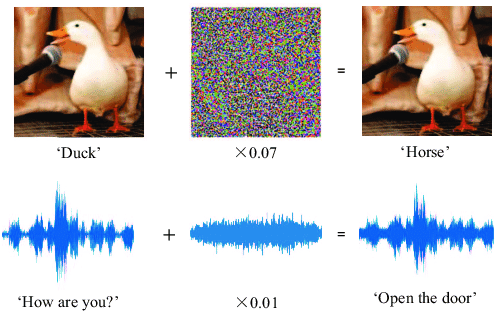
\includegraphics[scale=0.5]{pato}
    \end{figure}
    \pause
    \begin{center}
    How does adversarial training help our models ?
    \end{center}

  \end{frame}

  \begin{frame}{Adversarial examples creation techniques}

    \begin{itemize}
      \item Visual techniques: \citep{DBLP:journals/corr/abs-2005-05909}.\\
      \vspace{0.4cm}

      \begin{table}[H]
        \begin{tabular}{l|l|l}
        Original Input      & This film has a special place in my heart & \textcolor{green}{Positive} \\ \hline
        Adversarial example & This film has a special pl\textcolor{red}{ca}e in my he\textcolor{red}{ra}t & \textcolor{red}{Negative}
        \end{tabular}
        \caption{Example extracted from \citep{DBLP:journals/corr/abs-1801-04354}}
        \end{table}
      \item Semantic:\citep{DBLP:journals/corr/abs-1907-11932}.\\
        \vspace{0.4cm}
      \begin{figure}[H]
        \centering
        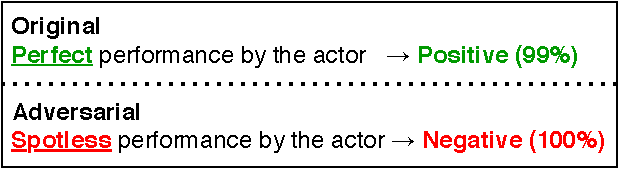
\includegraphics[scale=0.5]{00-ae-example}
        \caption{Example extracted from \citep{DBLP:journals/corr/abs-1907-11932}}
      \end{figure}

    \end{itemize}
  \end{frame}

  \begin{frame}{Our adversarial examples}
    Given a sequence of tokens \(s = \{x_1,\dots,x_T\}\)
    \begin{enumerate}
      \item We map each discrete token to an embedded representation in the continuous space
      \[
        \mathbf{E}x_i = e_i.  
      \]
      \item We add a little perturbation to the embedding
      \[
      e_i' = e_i - \epsilon \frac{\nabla_{e_i}J(s,\theta)}{\norm{\nabla_{e_i}J(s,\theta)}_2}.
      \]
      
    \end{enumerate}

    Current loss function:
    \[
    \mathcal J(\theta) = \sum_s \mathcal L(s,\theta) + \alpha \sum_{s'} \mathcal L_{adv} (s',\theta), \quad \alpha \in [0,1].  
    \]
  \end{frame}

  \subsection{Contrastive Learning}

  \begin{frame}{Contrastive Learning}
    
      %{\color{Maroon}\textbf{Idea}:} Pull the representations of positive examples (same class examples) close and push apart the representations of negative examples (rest of examples).
    

    \begin{ex}
      Original: Elephant. Positive: Tiger. Negative: Pizza.
    \end{ex}

    \begin{defi}[Contrastive loss]
      Let \(a_i\) be the original inputs, \(p_{a_i}\) positive examples and \(n_{a}\) negative examples. The contrastive loss is defined as follows:
      \[
      \mathcal L_{cont} = - \sum_{a_i \in A} \log \frac{\exp(a_i \cdot p_{a_i}/\tau)}{\sum_{n_a \in A - \{ a_i \} } \exp(a_i \cdot n_a / \tau)}  
      \]
    \end{defi}
  \end{frame}


  \section{Framework}

 

  \begin{frame}{Adversarial Training with Contrastive Learning (ATCL)}
    
    \setbeamercolor{background canvas}{bg=white}
    \begin{figure}
    \centering
    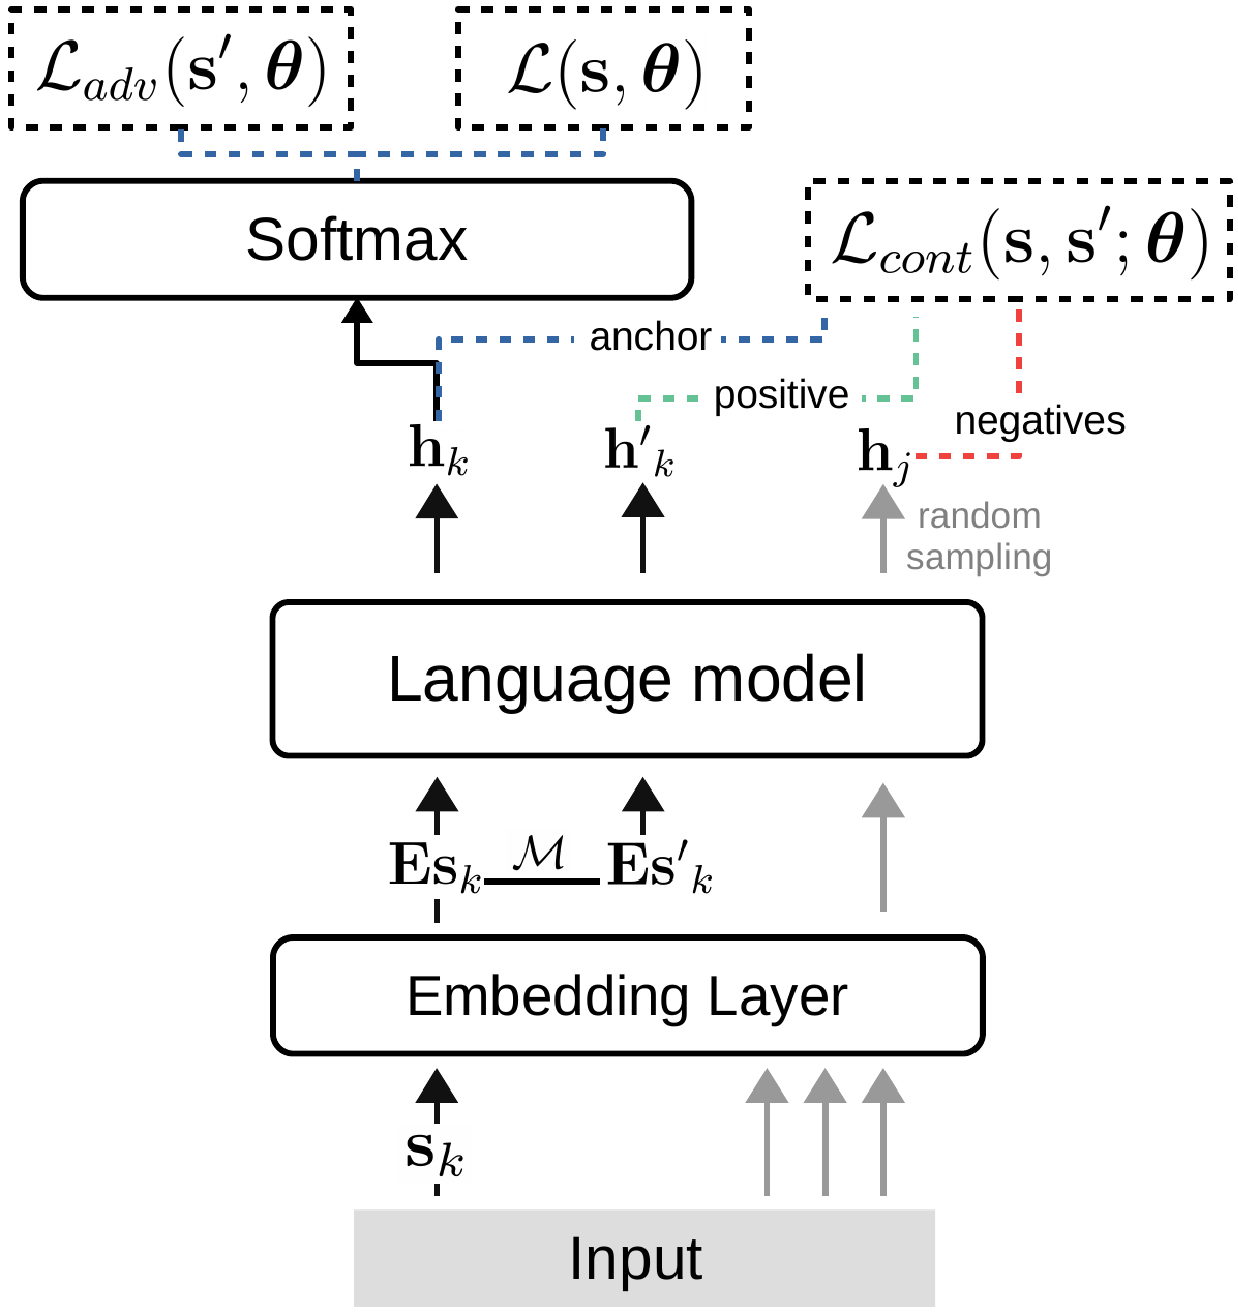
\includegraphics[scale=0.3]{embed}
    \caption{ACTL Framework. Image obtained from the original paper \citep{DBLP:journals/corr/abs-2109-09075}.}
    \end{figure}
  \end{frame}

  \begin{frame}{Considerations about ATCL}

    
    %\begin{itemize}
    %  \item We push apart the original sentence representation using the adversarial example, and we pull it back using the contrastive loss.
      
    %  \item In the contrastive loss, \(\mathcal L_{\text{cont}}\), the negative examples are sampled from the set \(\mathbf{H(S)} - \{h_{kj}\}\). This avoids sampling \(h_{kj}\) as a negative sample with itself.
    %\end{itemize}

    \begin{defi}[ATCL's loss function]
      The used loss function to train ATCL is:
      \[
      \mathcal J(\mathbf \theta)_{\text{ATCL}} =  \left( \mathcal L + \alpha \mathcal L_{\text{adv}} + \beta \mathcal L_{\text{cont}}\right)  
      \]
      \vspace{0.01cm}
    \end{defi}

    \end{frame}

  \section{Experiments and results}

  \begin{frame}{Language modeling}

\vspace{-0.3cm}
\begin{table}[t]
  \resizebox{\columnwidth}{!}{
\begin{tabular}{l|cccc}
\hline
\multirow{2}{*}{\textbf{Model and Training}} & \multicolumn{2}{c}{\textbf{Wikitext 103}} & \multicolumn{2}{c}{\textbf{Penn Tree Bank}} \\ \cline{2-5} 
 & \textbf{Validation}         & \textbf{Test}        & \textbf{Validation}          & \textbf{Test}         \\ \hline
\textbf{T XL base} & 23.10 & 24.00 & 56.72  & 54.52 \\ 
\textbf{T XL +TT}  & 23.61 &  25.70 & 57.90  & 55.40  \\ \hline
\textbf{Baseline TT} & 22.70 & 22.42 & 41.91 & 36.13 \\ 
\textbf{Baseline +Adv. only} & 21.75 & 21.67 & \textcolor{orange}{42.68} & \textcolor{orange}{36.46} \\ \hline
\textbf{Baseline +ATCL} (n=5) & 22.79 & 22.59 & 37.93 & 32.89\\ 
\textbf{Baseline +ATCL} (n=10) & 21.75 & 21.67 & \textbf{35.29} & \textbf{29.08} \\  
\textbf{Baseline +ATCL} (n=20) & \textbf{20.73} & \textbf{20.61} & 42.52 & 36.85 \\ 
\hline
\end{tabular}
}
	\caption{Perplexity achieved.}
	\label{tab:lmresults}
\end{table}

  \end{frame}


  \begin{frame}{Language modeling}

    \begin{table}[t]
\begin{center}
  \resizebox{\columnwidth}{!}{
    \begin{tabular}{c|c|c|c}
    \hline
    \textbf{Word}   & \textbf{Baseline}      & \textbf{+Adv. only  }    & \textbf{+ATCL}    \\ \hline
    \textbf{friend} & \makecell{`brother', `daughter', \\ `understanding', \textbf{`director'}} & \makecell{`cousin', `colleague', \\ \textbf{`knowledge'}, `mentor'} & \makecell{`cousin', `fellow', \\ `partner', `colleague'} \\ \hline
    \textbf{hate}   & \makecell{`admit', `prejudice', \\ `troubled', `regret'} & \makecell{\textbf{`loving'}, `hurt', \\ \textbf{`embrace'}, `committing' } & \makecell{`dirty', `poison', \\ `regret', `shame'} \\ \hline
    \end{tabular}
  }
	\caption{Four closest neighbors of some words in the vocabulary of the WikiText-103. Table from \citep{DBLP:journals/corr/abs-2109-09075}. }
    \label{tab:lmneigh}
\end{center}
\end{table}
  \end{frame}

  \begin{frame}{Neural Machine Translation}
\begin{table}[ht]
\begin{center}
\resizebox{\columnwidth}{!}{
\begin{tabular}{|l|c|c|c|c|}
\hline
\textbf{Model name}   & \textbf{En-De} & \textbf{De-En} & \textbf{En-Fr} & \textbf{Fr-En} \\ \hline
\begin{tabular}[l]{@{}l@{}}\textbf{Baseline} \\ \textbf{(Transformer S)}\end{tabular} & 24.61 & 30.34 & 35.23 & 34.51 \\ \hline
\textbf{Baseline +Adv} & 25.04 & 30.36  & 35.02 & \textbf{35.97} \\ \hline
\multirow{3}{*}{\textbf{Baseline +ATCL}}  & 24.63 & \textbf{31.34} & \textbf{36.40} & 35.35 \\ \cline{2-5} 
 & \textbf{25.26} & 30.36 & 35.60  & 35.48 \\ \cline{2-5} 
    & 24.74 & 30.13  & 35.38 & 35.46 \\ \hline
\end{tabular}
}
	\caption{BLEU test scores for the IWSLT dataset. Table from \citep{DBLP:journals/corr/abs-2109-09075}.}
    \label{tab:nmtresults}
\end{center}
\end{table}
\end{frame}

  
  \begin{frame}{Conclusions}

    \begin{itemize}
      \item Usage of two general machine learning techniques applied to natural language processing.
      \item Applying this method has a similar effect to regularization.
      \item Results are promising in Language modeling, but not so much in Neural Machine Translation.
    \end{itemize}
  \end{frame}
  
  \appendix

  \begin{frame}[noframenumbering,standout]
    Thank you for your attention.
  \end{frame}


  \begin{frame}[noframenumbering]

  \vspace{0.5cm}
  \bibliographystyle{dinat}
  \bibliography{bibliography.bib}

  \end{frame}

   \begin{frame}[noframenumbering]{Elements}
    We consider:
    
    \begin{itemize}
    \item  \(\mathbf S = \{s_1,\dots,s_B\}\) a set of sentences, where each sentence \(s_k = \{x_{k1},\dots,x_{kN}\}\) contains \(N\) tokens.
    \item \(\mathbf E s_k = \{\mathbf E x_{k1},\dots, \mathbf E x_{kN}\} = \{e_{k1},\dots e_{kN}\}\) the continuous space embedding of each sentence.
    \item The vocabulary \(\mathcal V\) and a \textbf{restricted} subset from it in which we exclude incomplete words (single characters or symbols) \(\mathcal V_R\)
    \item The restriction function from \(\mathcal V\) to \(\mathcal V_R\):
    \[
      \mathcal M (\mathbf E x_{ki}) = \begin{cases}1 & \text{ if } x_{ki}\in \mathcal V_R \\ 0 & \text{otherwise}\end{cases}
    \]
    (this function avoids taking senseless adversarial candidates).

    \item  \(h_{kj}\) the representation of each sentence \(s_k\).

    \end{itemize}
  \end{frame}

\end{document}
